
\documentclass{beamer}

\usepackage[utf8]{inputenc}
\usepackage{graphicx}
%\usepackage{amsmath}
\graphicspath{ {./images/} }
\usepackage{subcaption}

\usepackage{enumitem}
\setlist{itemsep=10pt}
\setitemize{label=\usebeamerfont*{itemize item}%
  \usebeamercolor[fg]{itemize item}
  \usebeamertemplate{itemize item}}

%Information to be included in the title page:
\title{Stabilization Flipbook}
%\author{Anonymous}
%\institute{ShareLaTeX}
\date{2018}

\begin{document}
\frame{\titlepage}


\begin{frame}
  \begin{figure}[h!]
    \centering
      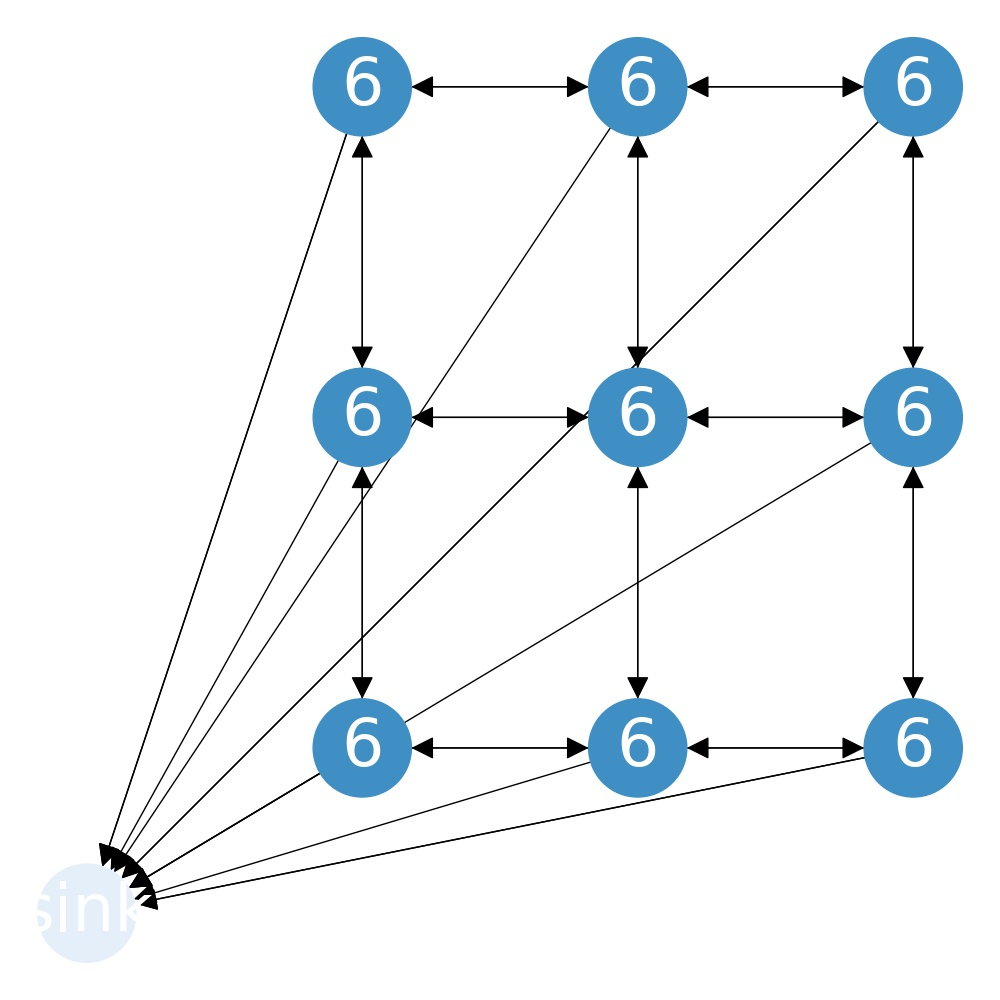
\includegraphics[scale=0.25]{sandpile_0}
  \end{figure}
\end{frame}


\begin{frame}
  \begin{figure}[h!]
    \centering
      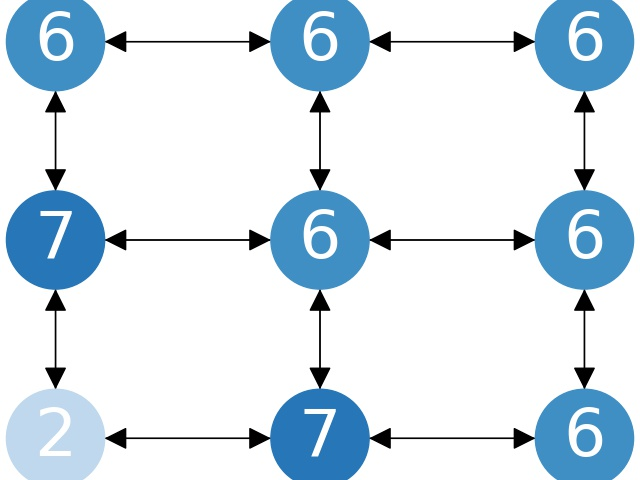
\includegraphics[scale=0.25]{sandpile_1}
  \end{figure}
\end{frame}


\begin{frame}
  \begin{figure}[h!]
    \centering
      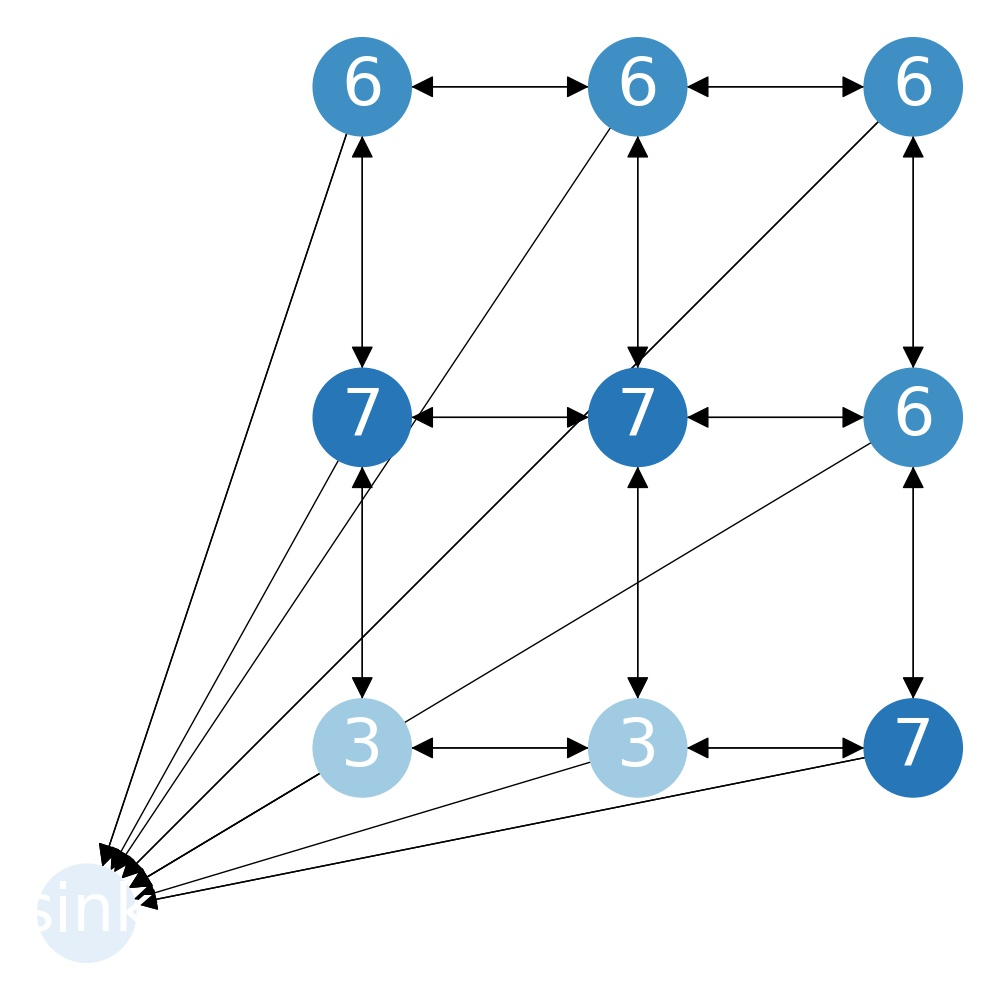
\includegraphics[scale=0.25]{sandpile_2}
  \end{figure}
\end{frame}


\begin{frame}
  \begin{figure}[h!]
    \centering
      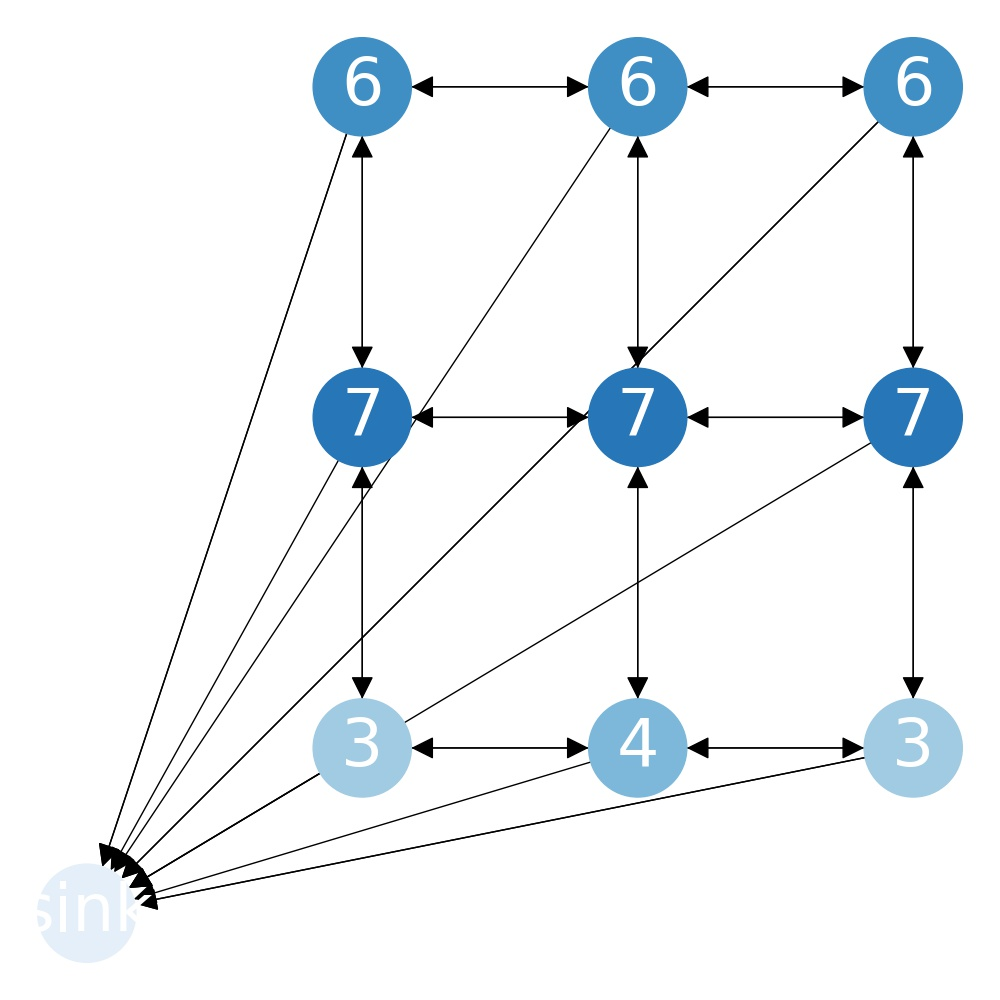
\includegraphics[scale=0.25]{sandpile_3}
  \end{figure}
\end{frame}


\begin{frame}
  \begin{figure}[h!]
    \centering
      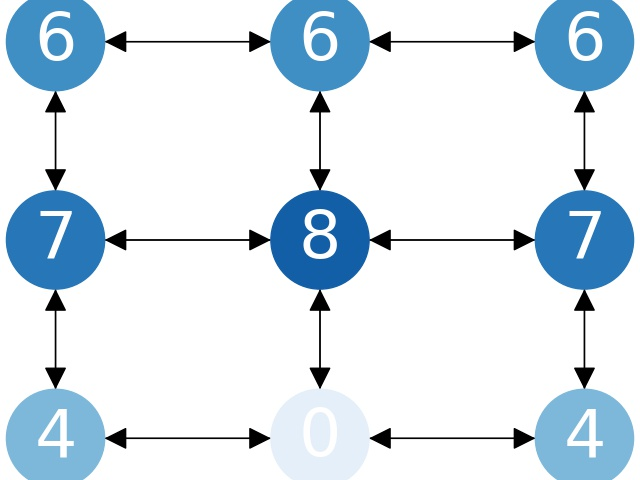
\includegraphics[scale=0.25]{sandpile_4}
  \end{figure}
\end{frame}


\begin{frame}
  \begin{figure}[h!]
    \centering
      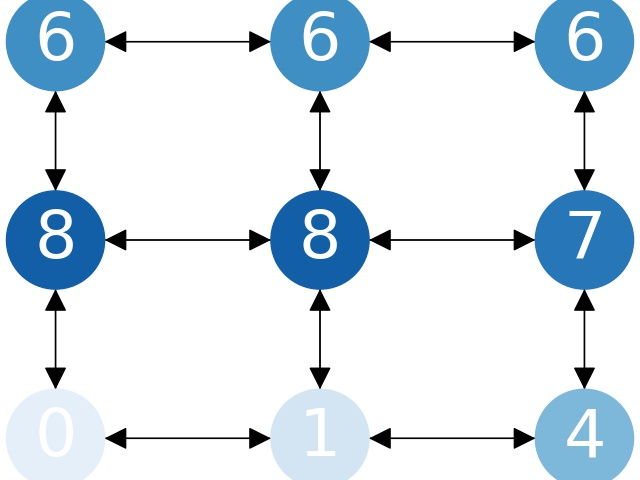
\includegraphics[scale=0.25]{sandpile_5}
  \end{figure}
\end{frame}


\begin{frame}
  \begin{figure}[h!]
    \centering
      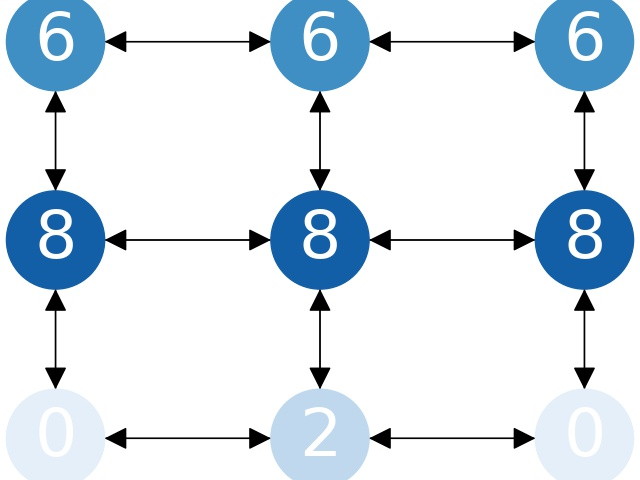
\includegraphics[scale=0.25]{sandpile_6}
  \end{figure}
\end{frame}


\begin{frame}
  \begin{figure}[h!]
    \centering
      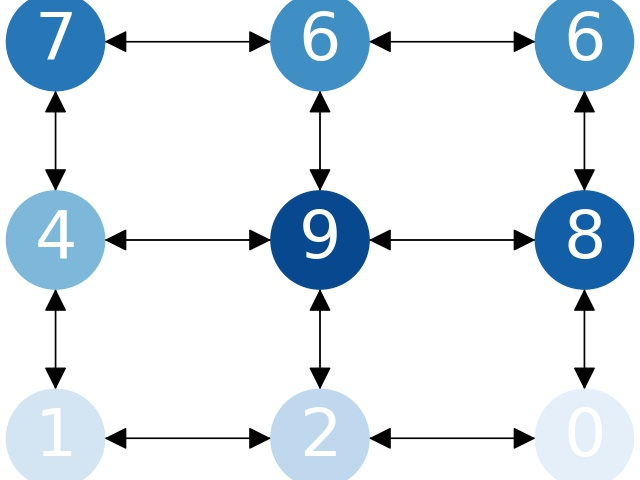
\includegraphics[scale=0.25]{sandpile_7}
  \end{figure}
\end{frame}


\begin{frame}
  \begin{figure}[h!]
    \centering
      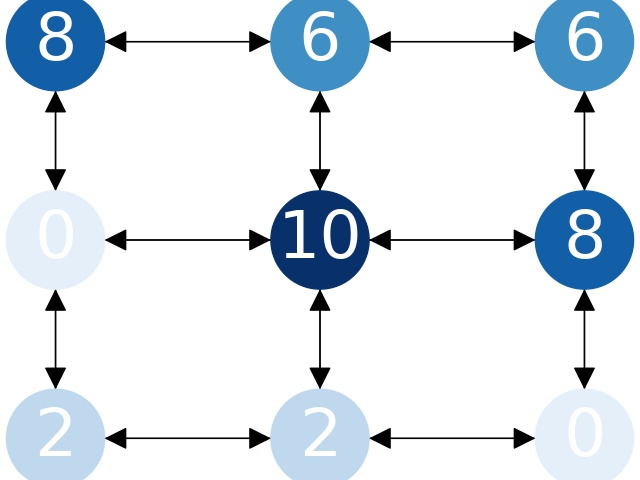
\includegraphics[scale=0.25]{sandpile_8}
  \end{figure}
\end{frame}


\begin{frame}
  \begin{figure}[h!]
    \centering
      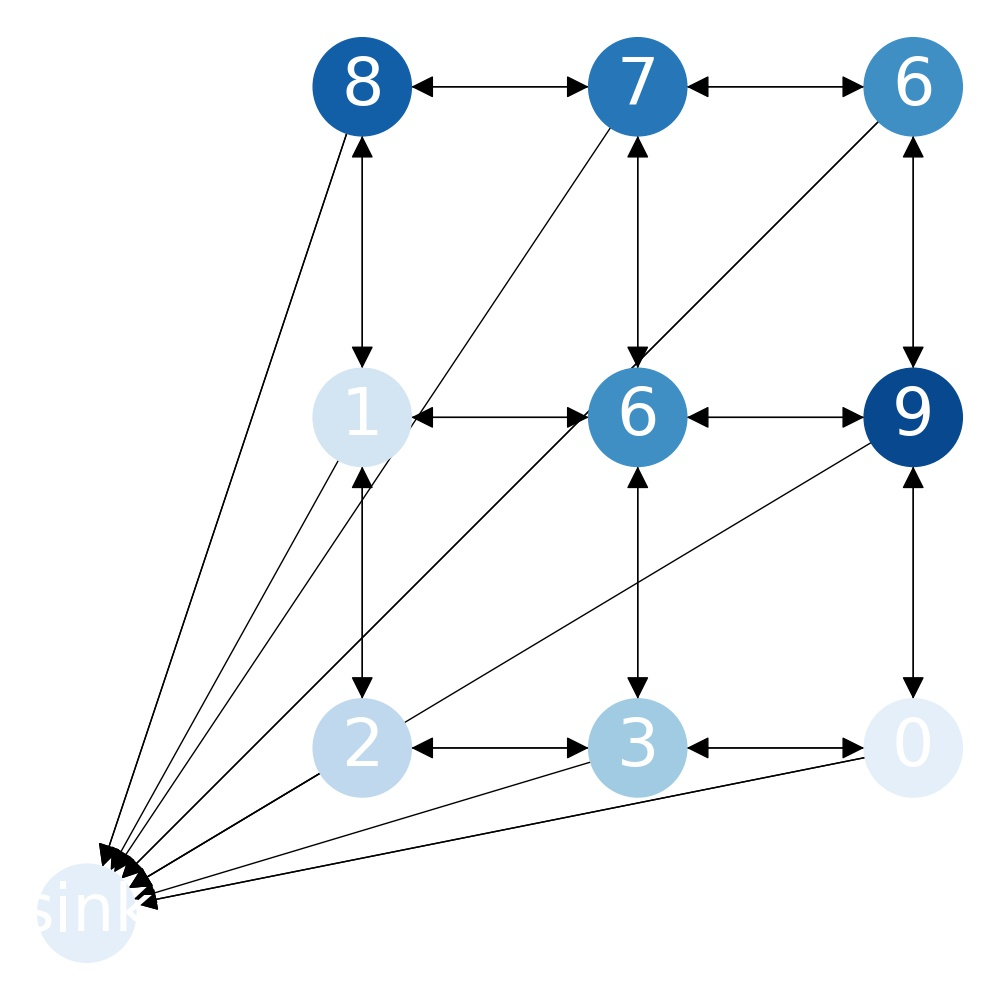
\includegraphics[scale=0.25]{sandpile_9}
  \end{figure}
\end{frame}


\begin{frame}
  \begin{figure}[h!]
    \centering
      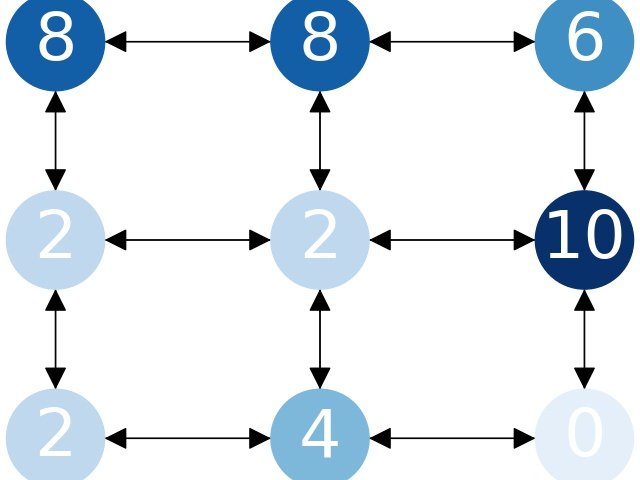
\includegraphics[scale=0.25]{sandpile_10}
  \end{figure}
\end{frame}


\begin{frame}
  \begin{figure}[h!]
    \centering
      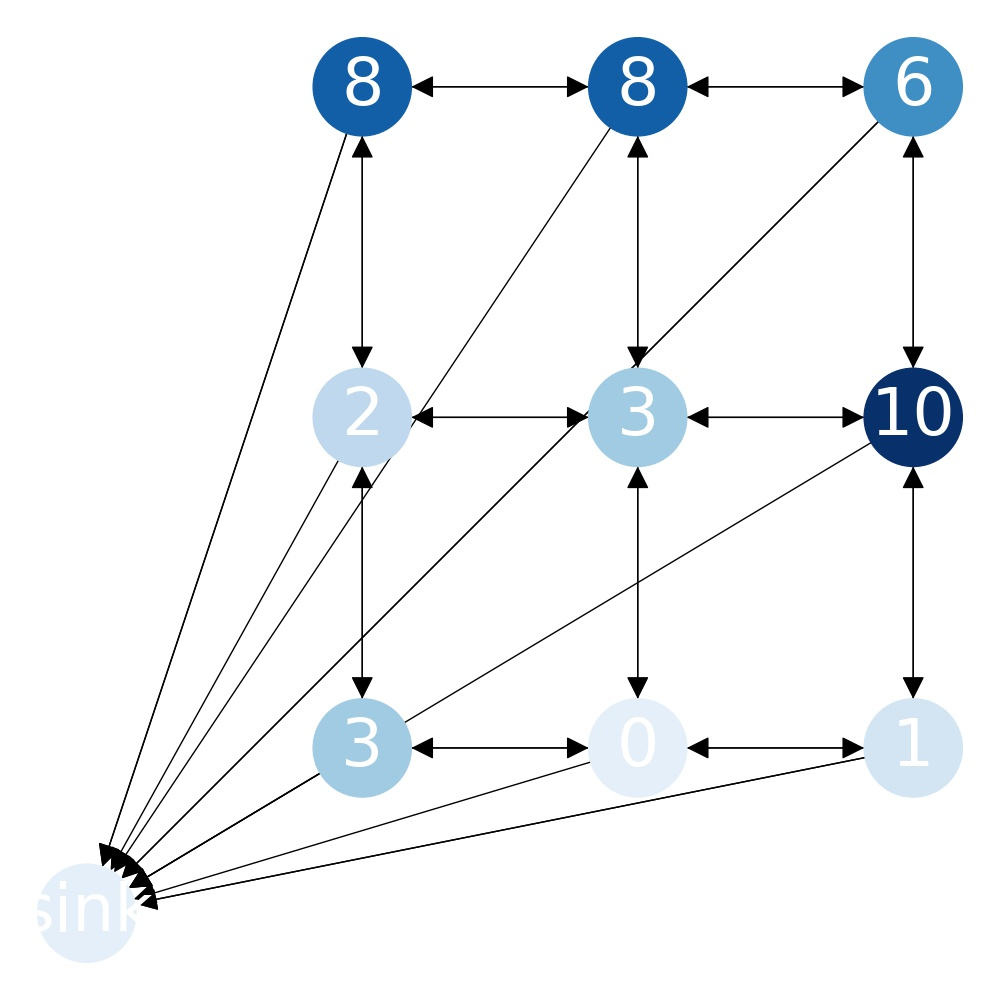
\includegraphics[scale=0.25]{sandpile_11}
  \end{figure}
\end{frame}


\begin{frame}
  \begin{figure}[h!]
    \centering
      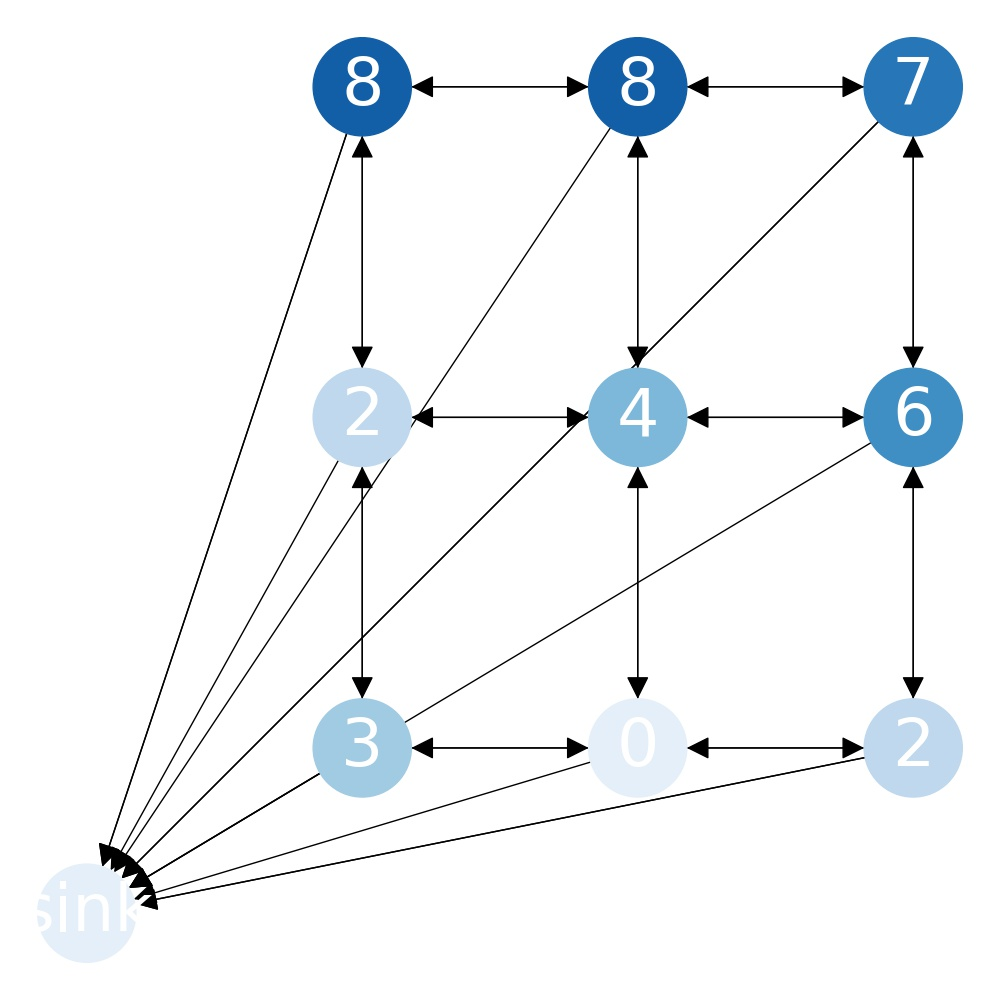
\includegraphics[scale=0.25]{sandpile_12}
  \end{figure}
\end{frame}


\begin{frame}
  \begin{figure}[h!]
    \centering
      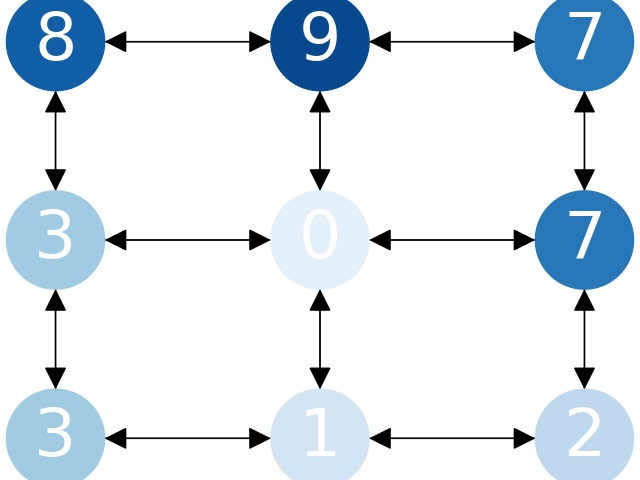
\includegraphics[scale=0.25]{sandpile_13}
  \end{figure}
\end{frame}


\begin{frame}
  \begin{figure}[h!]
    \centering
      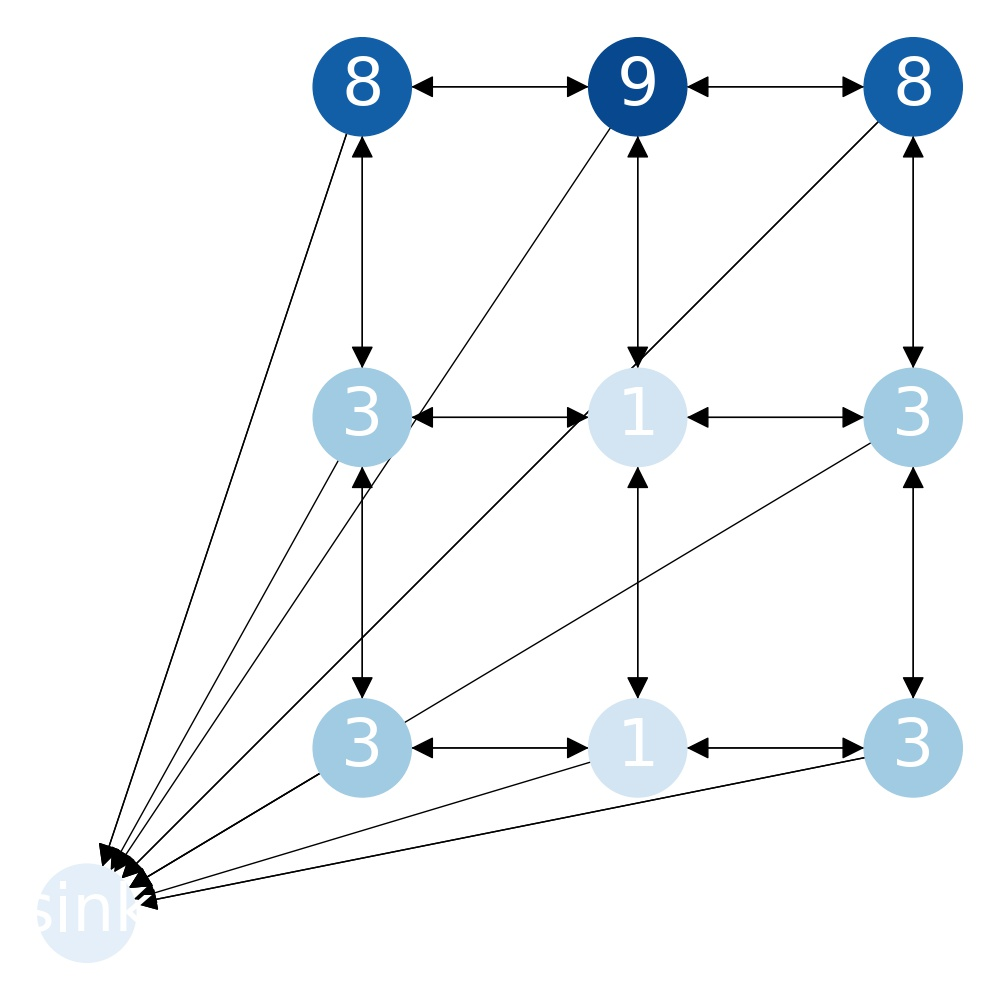
\includegraphics[scale=0.25]{sandpile_14}
  \end{figure}
\end{frame}


\begin{frame}
  \begin{figure}[h!]
    \centering
      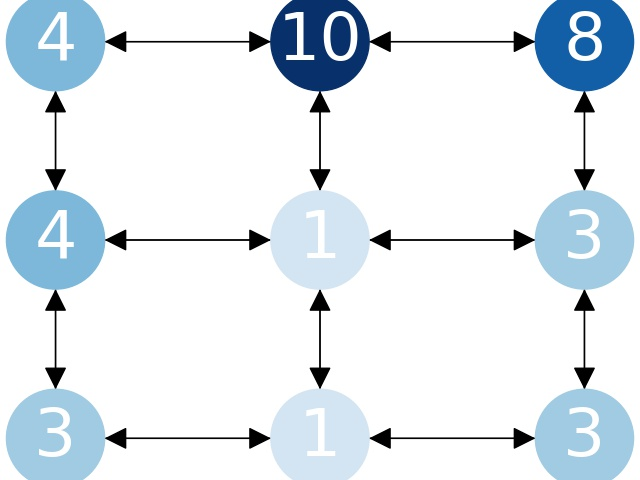
\includegraphics[scale=0.25]{sandpile_15}
  \end{figure}
\end{frame}


\begin{frame}
  \begin{figure}[h!]
    \centering
      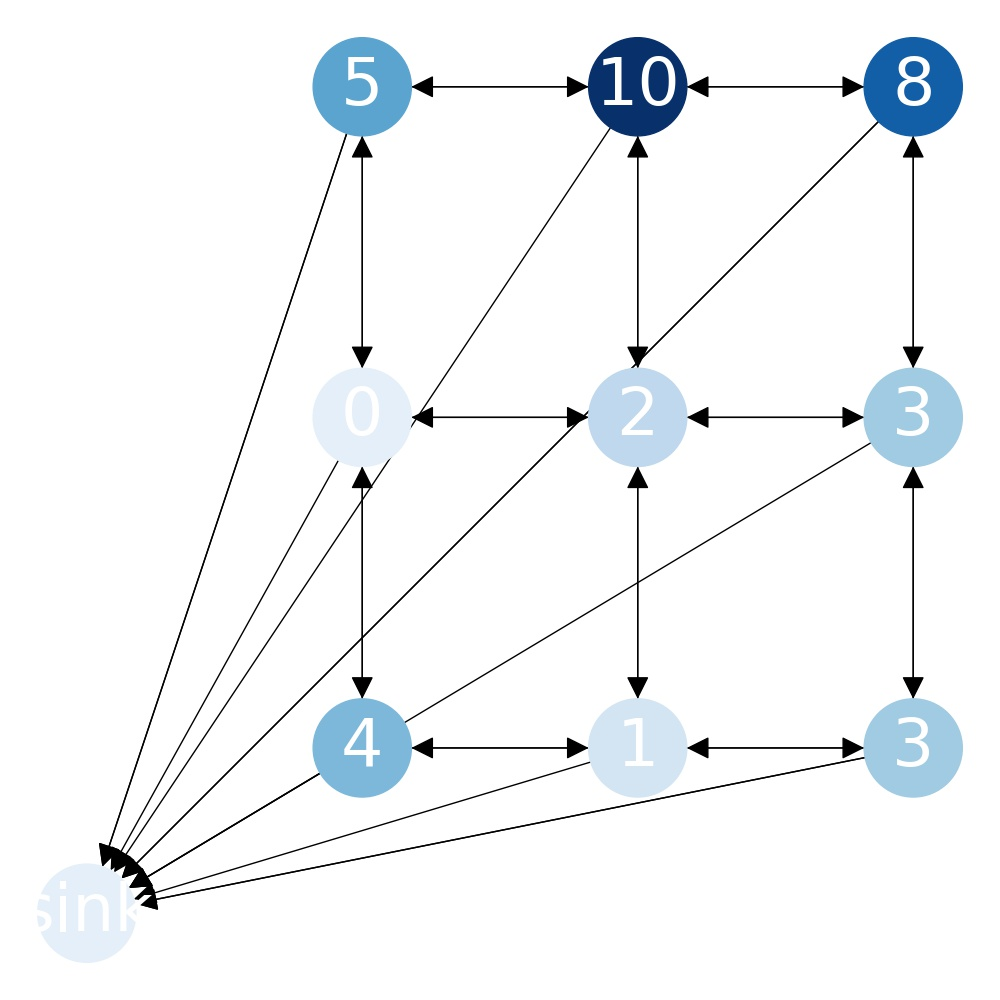
\includegraphics[scale=0.25]{sandpile_16}
  \end{figure}
\end{frame}


\begin{frame}
  \begin{figure}[h!]
    \centering
      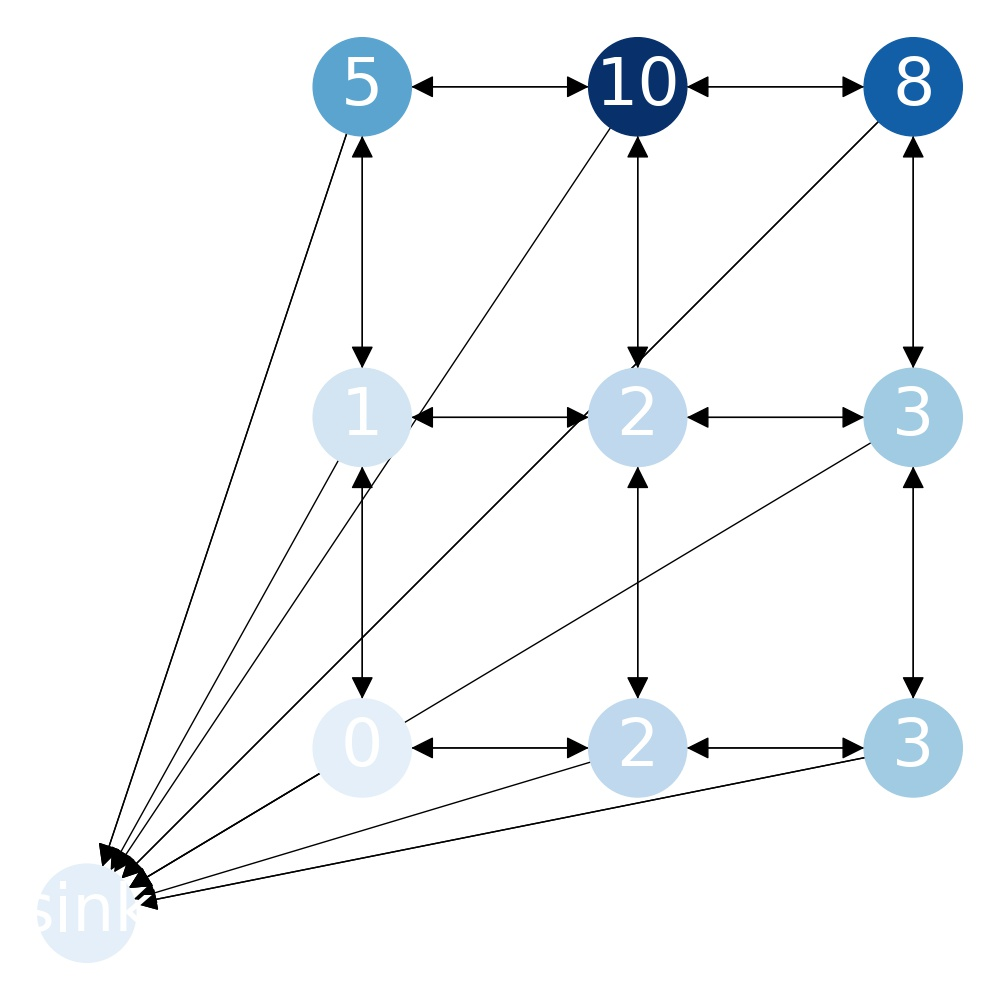
\includegraphics[scale=0.25]{sandpile_17}
  \end{figure}
\end{frame}


\begin{frame}
  \begin{figure}[h!]
    \centering
      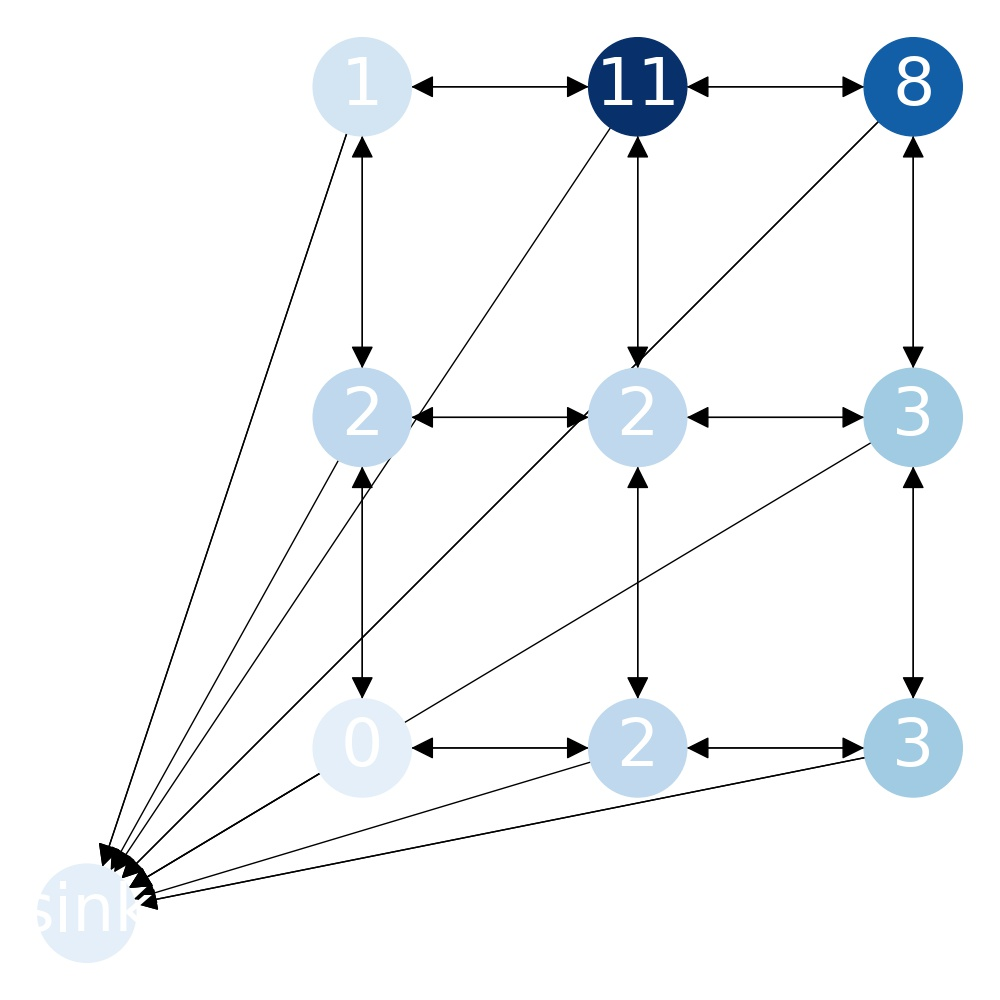
\includegraphics[scale=0.25]{sandpile_18}
  \end{figure}
\end{frame}


\begin{frame}
  \begin{figure}[h!]
    \centering
      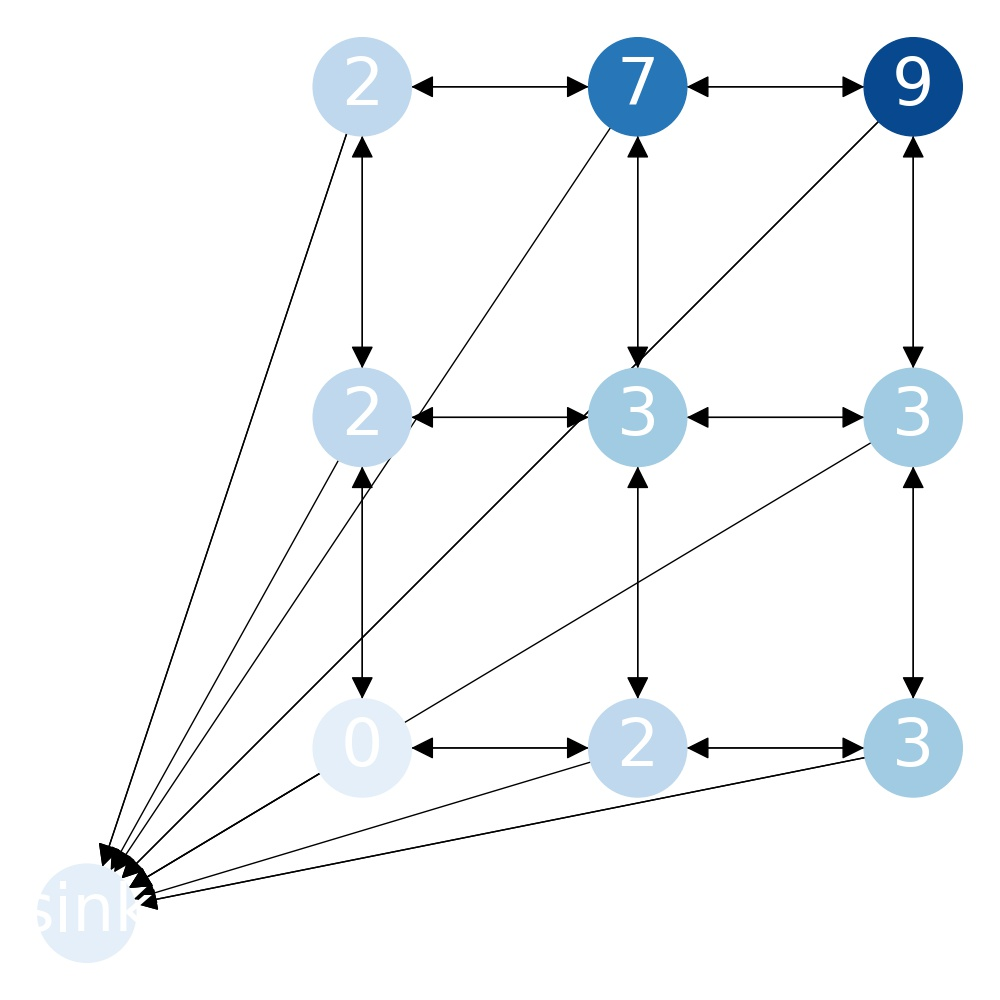
\includegraphics[scale=0.25]{sandpile_19}
  \end{figure}
\end{frame}


\begin{frame}
  \begin{figure}[h!]
    \centering
      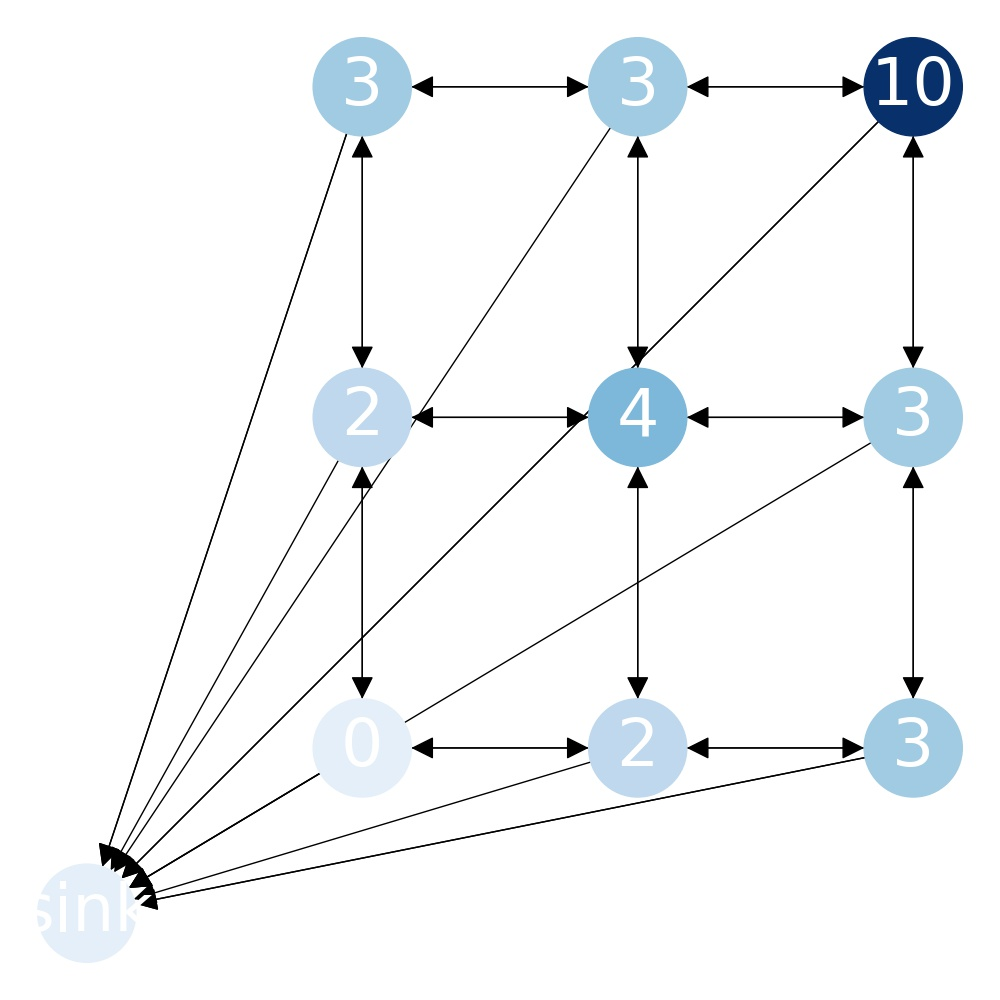
\includegraphics[scale=0.25]{sandpile_20}
  \end{figure}
\end{frame}


\begin{frame}
  \begin{figure}[h!]
    \centering
      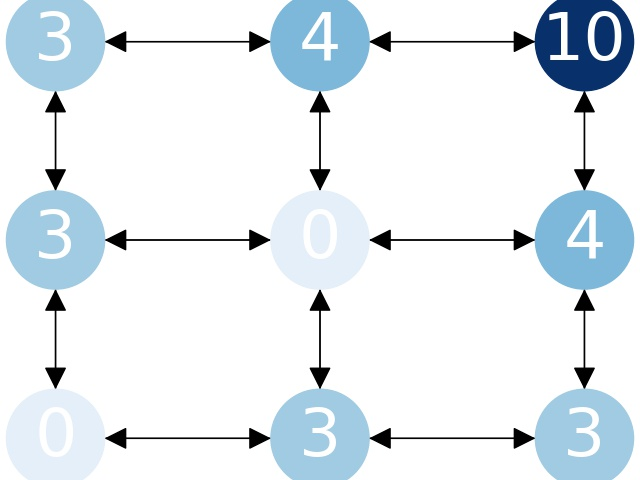
\includegraphics[scale=0.25]{sandpile_21}
  \end{figure}
\end{frame}


\begin{frame}
  \begin{figure}[h!]
    \centering
      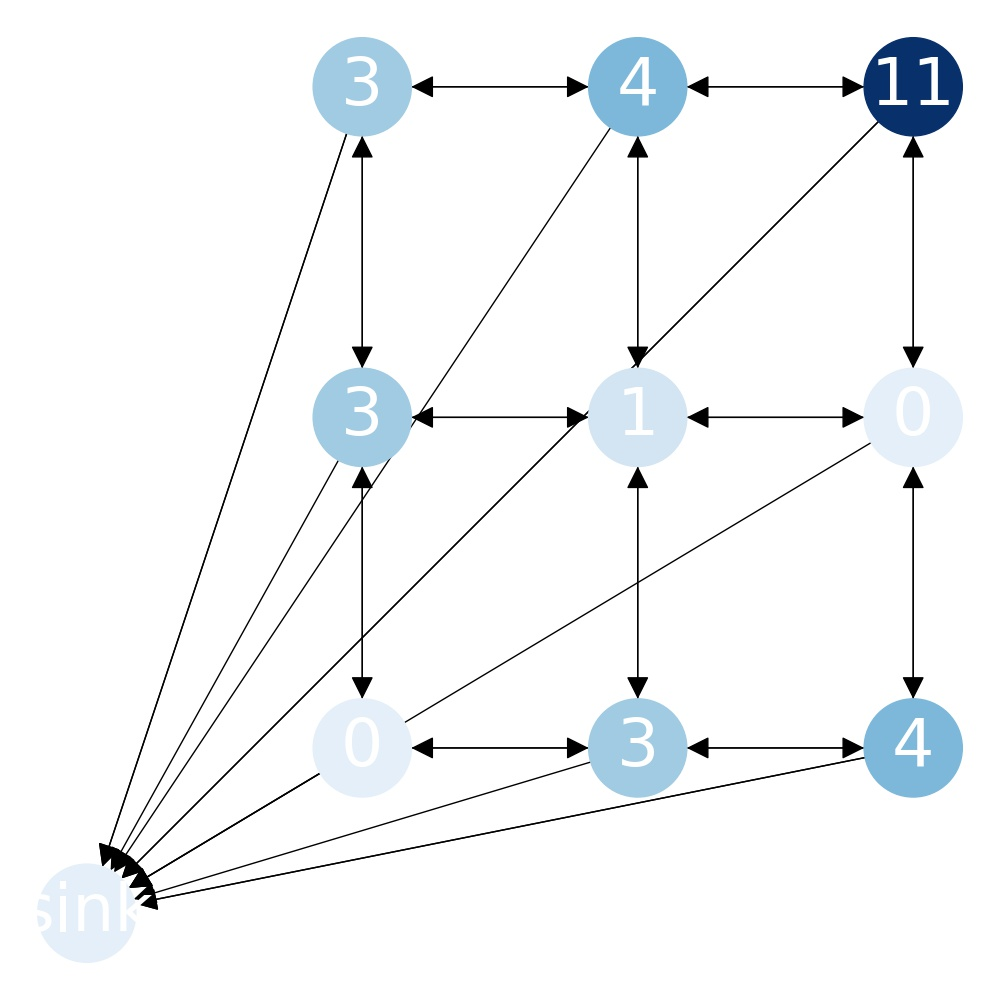
\includegraphics[scale=0.25]{sandpile_22}
  \end{figure}
\end{frame}


\begin{frame}
  \begin{figure}[h!]
    \centering
      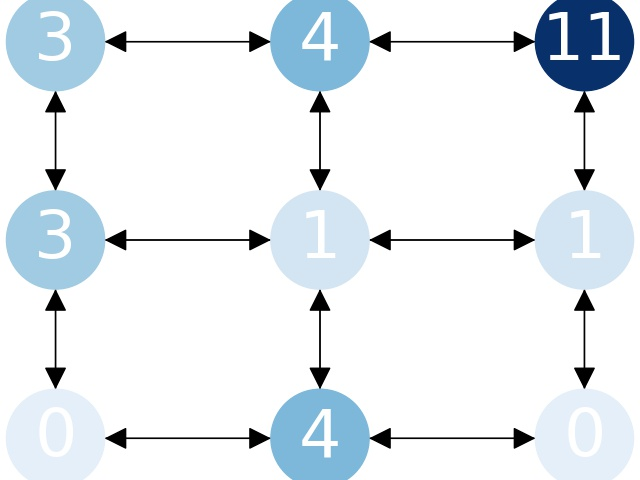
\includegraphics[scale=0.25]{sandpile_23}
  \end{figure}
\end{frame}


\begin{frame}
  \begin{figure}[h!]
    \centering
      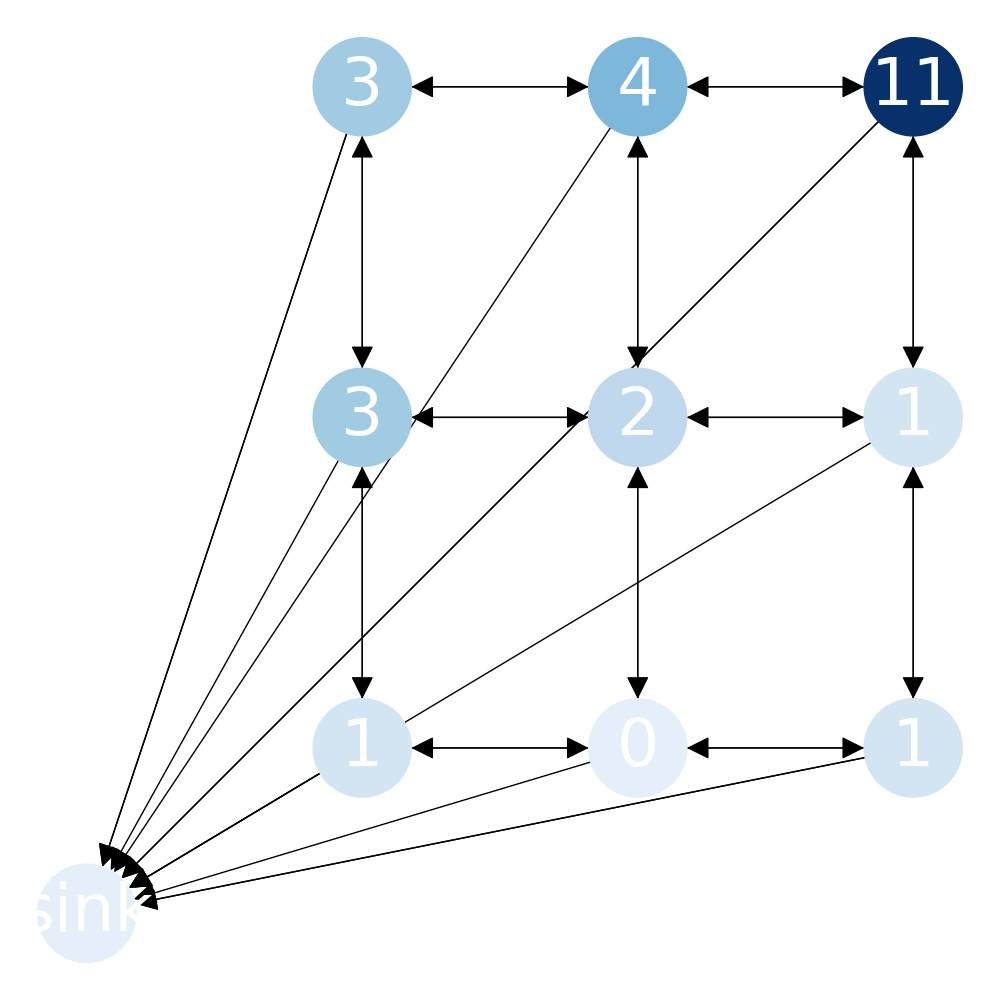
\includegraphics[scale=0.25]{sandpile_24}
  \end{figure}
\end{frame}


\begin{frame}
  \begin{figure}[h!]
    \centering
      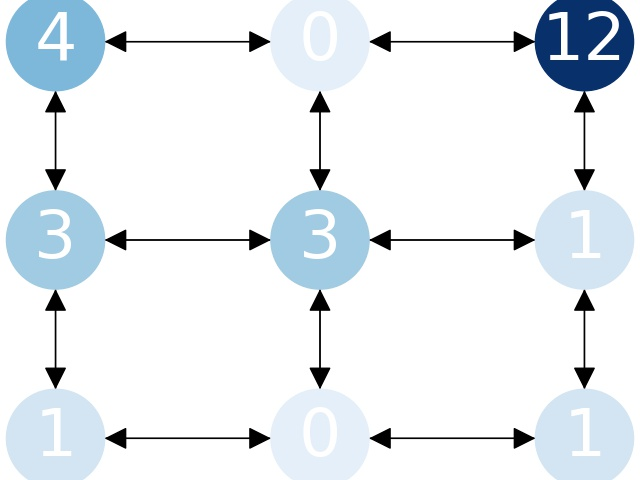
\includegraphics[scale=0.25]{sandpile_25}
  \end{figure}
\end{frame}


\begin{frame}
  \begin{figure}[h!]
    \centering
      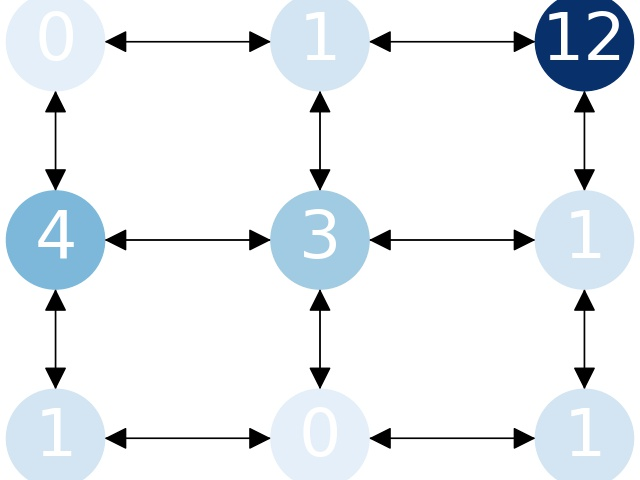
\includegraphics[scale=0.25]{sandpile_26}
  \end{figure}
\end{frame}


\begin{frame}
  \begin{figure}[h!]
    \centering
      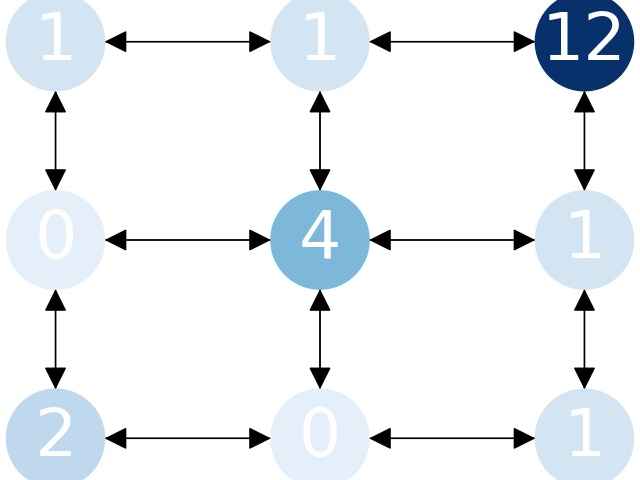
\includegraphics[scale=0.25]{sandpile_27}
  \end{figure}
\end{frame}


\begin{frame}
  \begin{figure}[h!]
    \centering
      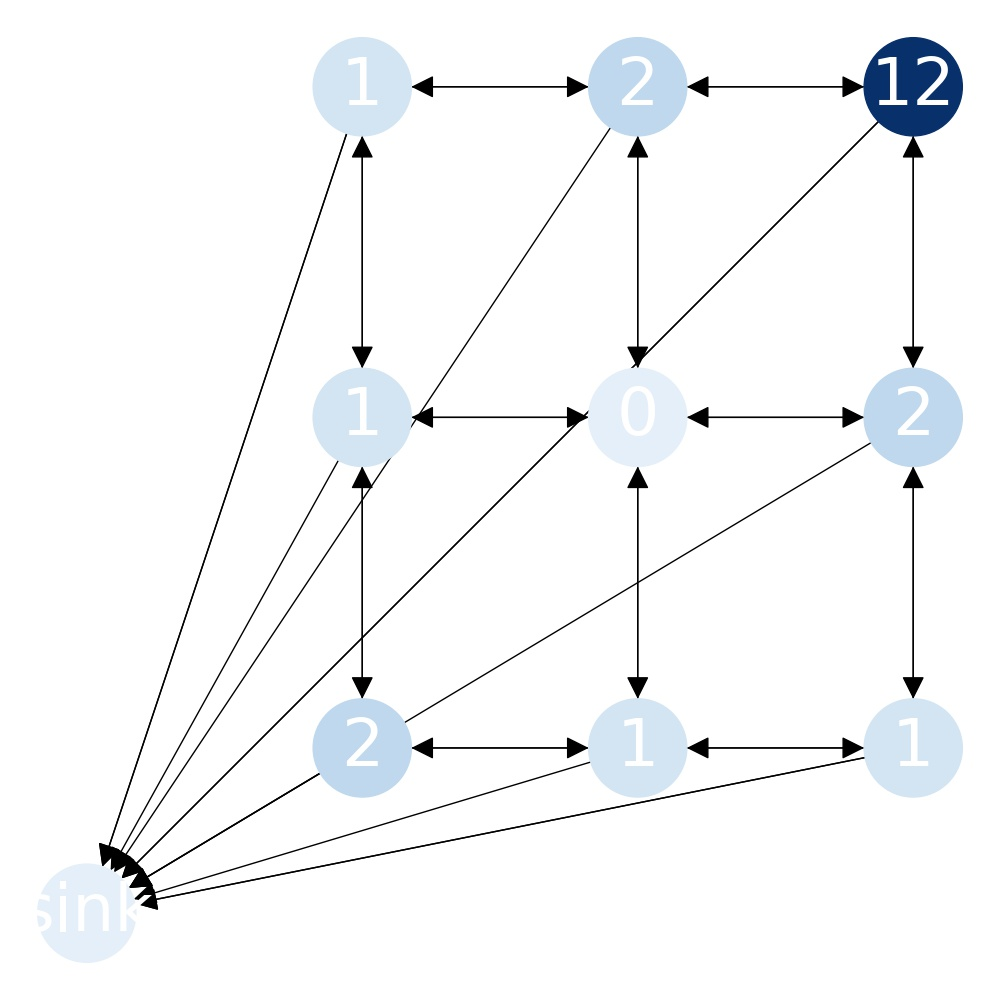
\includegraphics[scale=0.25]{sandpile_28}
  \end{figure}
\end{frame}


\begin{frame}
  \begin{figure}[h!]
    \centering
      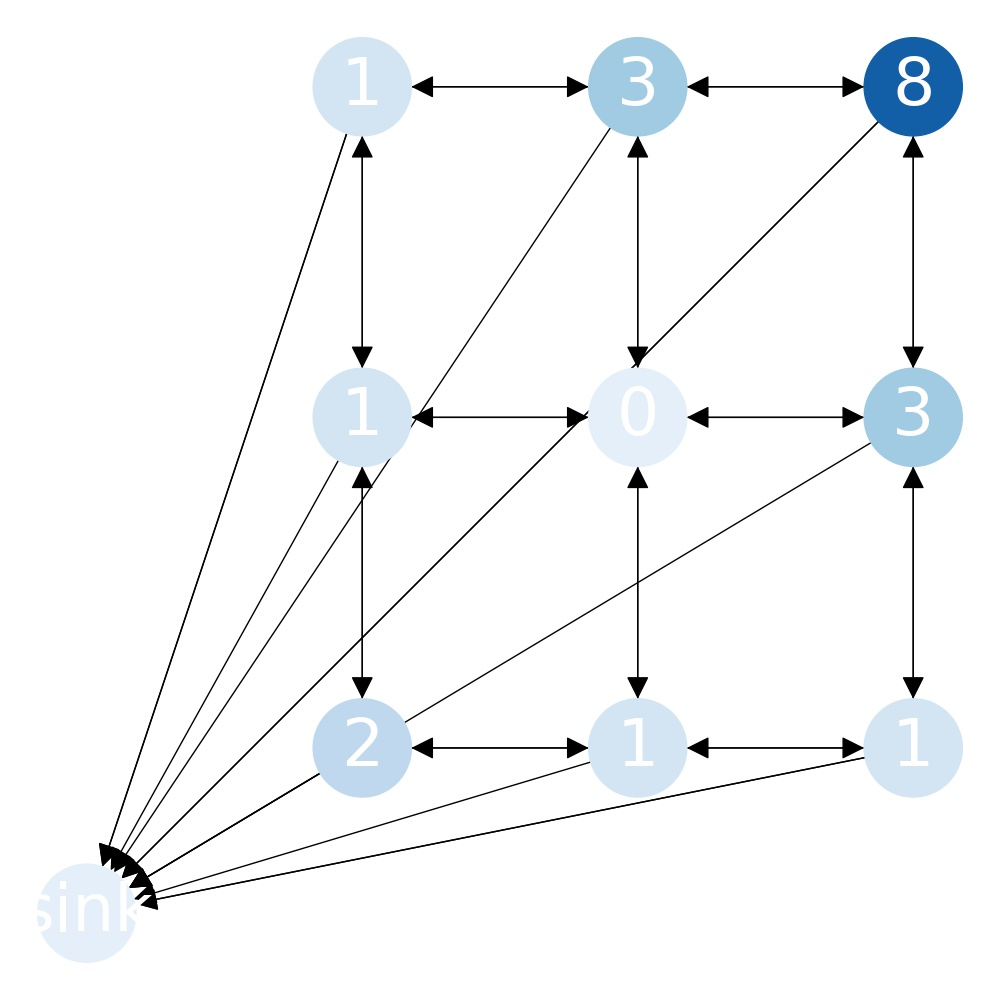
\includegraphics[scale=0.25]{sandpile_29}
  \end{figure}
\end{frame}


\begin{frame}
  \begin{figure}[h!]
    \centering
      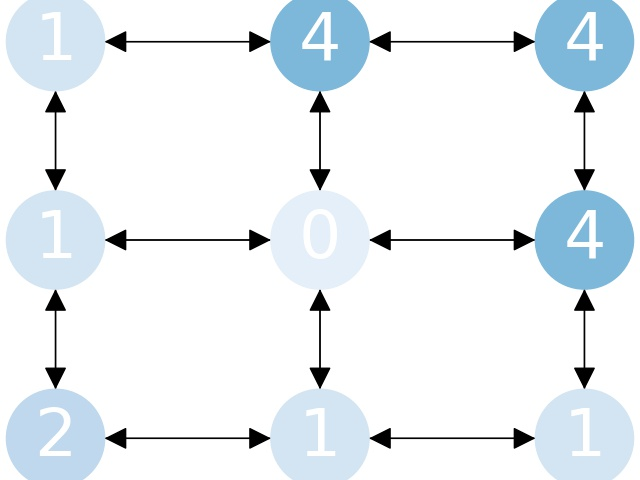
\includegraphics[scale=0.25]{sandpile_30}
  \end{figure}
\end{frame}


\begin{frame}
  \begin{figure}[h!]
    \centering
      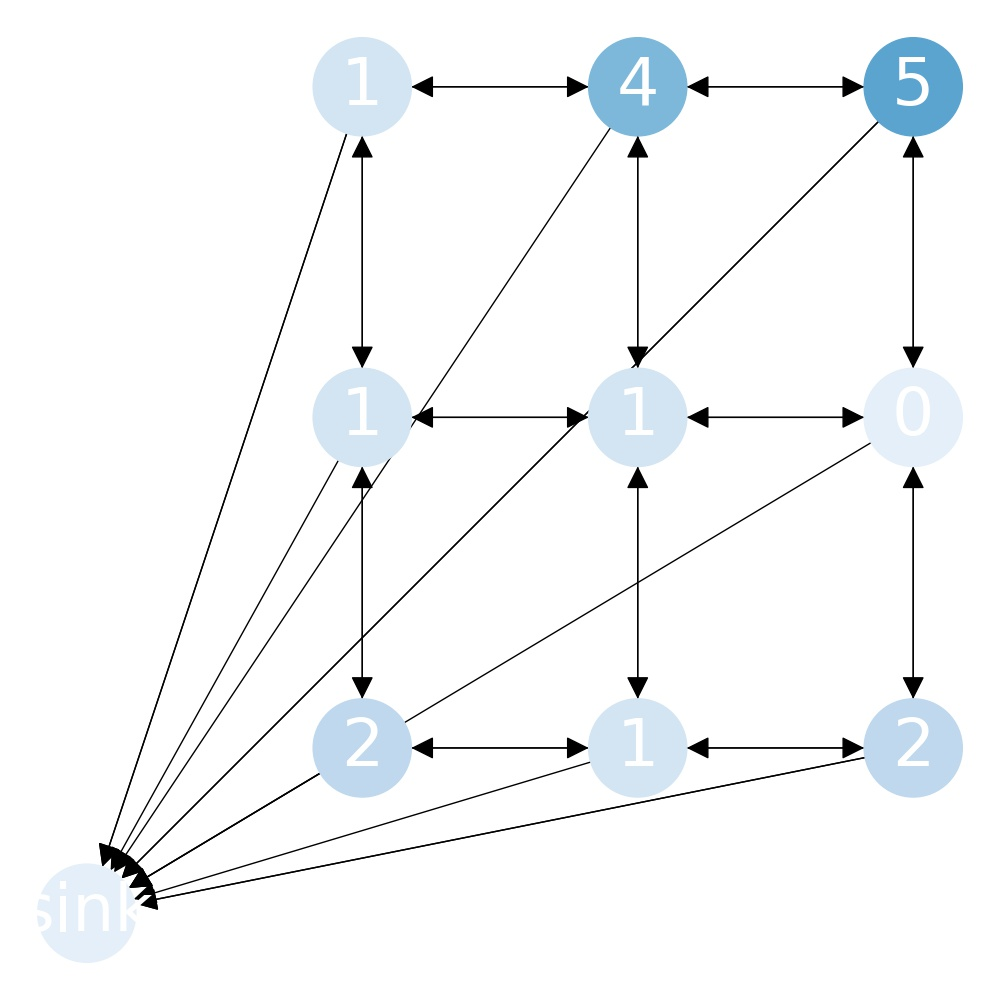
\includegraphics[scale=0.25]{sandpile_31}
  \end{figure}
\end{frame}


\begin{frame}
  \begin{figure}[h!]
    \centering
      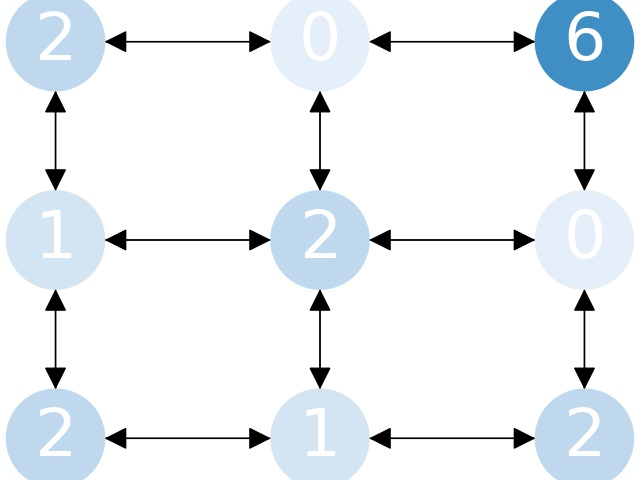
\includegraphics[scale=0.25]{sandpile_32}
  \end{figure}
\end{frame}


\begin{frame}
  \begin{figure}[h!]
    \centering
      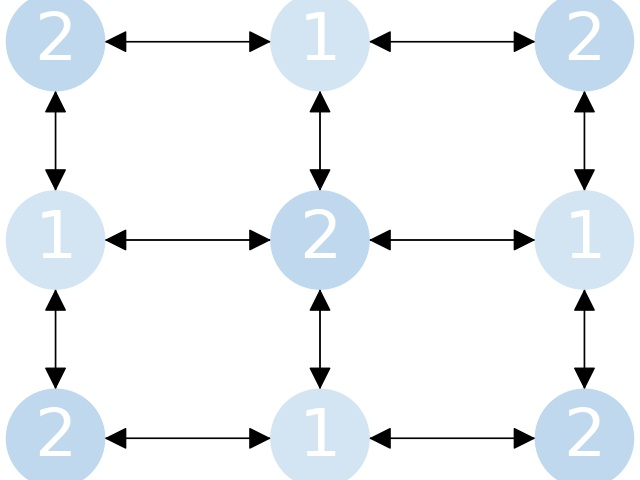
\includegraphics[scale=0.25]{sandpile_33}
  \end{figure}
\end{frame}


\begin{frame}

[0, 1, 2, 1, 0, 2, 3, 3, 4, 4, 1, 5, 4, 5, 6, 3, 0, 6, 7, 7, 4, 5, 2, 1, 7, 6, 3, 4, 8, 8, 5, 7, 8]

\[
\{{0: 3, 1: 4, 2: 3, 3: 4, 4: 5, 5: 4, 6: 3, 7: 4, 8: 3}\}
\]
\end{frame}


\end{document}
